
\noindent\textbf{Simulations}
%
Despite large amounts of noise introduced into the simulated measurements, and
the missing observations, both the Kalman filter and smoother yielded accurate
estimates of true positions.
%
The Kalman filter and smoother provided more accurate estimates of velocities
and accelerations than the baseline finite differences method.
%
We also obtained more accurate estimates with learned than with manually set
parameters.
%
For missing observations, estimates by the Kalman smoother were more accurate
than those by the Kalman filter.

\noindent\textbf{Mouse tracking}
%
The interactive figure shows positions extracted with the computer vision
functions and those inferred by the Kalman filter and smoother, for an example
session. At times with missing observations (i.e., missing black dots) the
Kalman smoother provided better position estimates than the Kalman filter, that
sometimes went astray.
% 
As with simulated data, estimates of velocities and acceleration by the
baseline finite differences method appeared substantially noisier than those
from the Kalman filter and smoother (data not shown). Extrapolating from the
simulation results, we infer that for behaving mice velocity and acceleration
estimates are more accurate for the Kalman filter and smoother than for the
finite difference method.

\begin{figure}
    \begin{center}

        \href{http://www.gatsby.ucl.ac.uk/~rapela/fwg/reports/learning/figures/positions_smoothed_session003_start0.00_end15548.27_startPosition0_numPosition10000_pos_learnedParams.html}{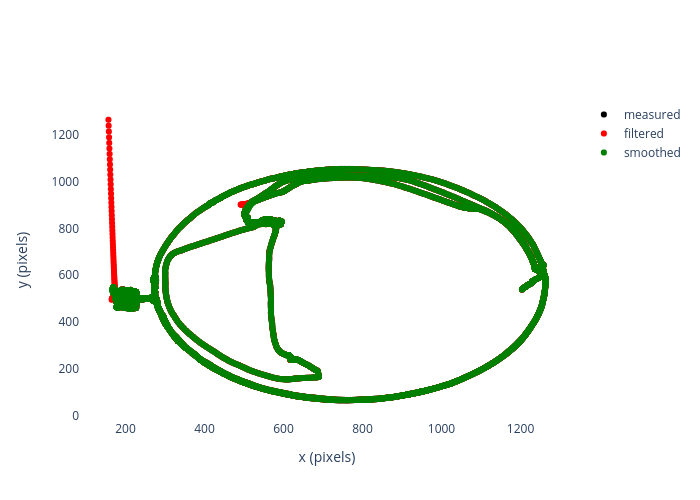
\includegraphics[width=3in]{{figures/positions_smoothed_session003_start0.00_end15548.27_startPosition0_numPosition10000_pos_learnedParams}.png}}

        \caption{Positions measured with computer vision functions (black) or
        inferred with the Kalman filter (red) or smoothing (green) algorithm.
        Parameters of the LDS used for inference were learned from data.
        Please refer to \cite{c3} for an interactive version of this figure,
        and double click on a trace legend to hide/show the corresponding
        trace.}

    \end{center}
\end{figure}

